% Created by tikzDevice version 0.12.3 on 2020-05-24 18:12:23
% !TEX encoding = UTF-8 Unicode
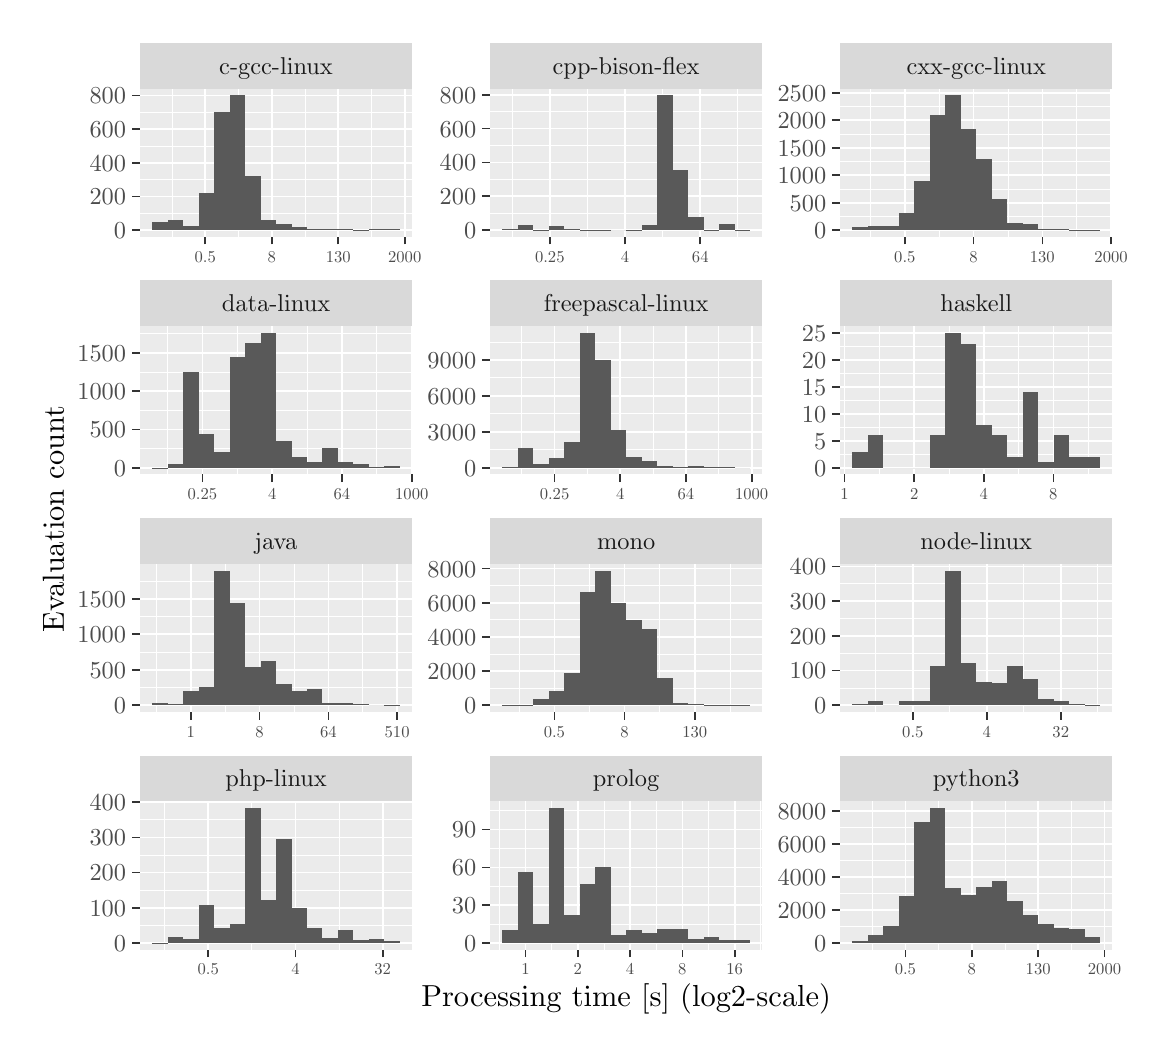
\begin{tikzpicture}[x=1pt,y=1pt]
\definecolor{fillColor}{RGB}{255,255,255}
\path[use as bounding box,fill=fillColor,fill opacity=0.00] (0,0) rectangle (397.48,361.35);
\begin{scope}
\path[clip] (  0.00,  0.00) rectangle (397.48,361.35);
\definecolor{drawColor}{RGB}{255,255,255}
\definecolor{fillColor}{RGB}{255,255,255}

\path[draw=drawColor,line width= 0.6pt,line join=round,line cap=round,fill=fillColor] (  0.00,  0.00) rectangle (397.48,361.35);
\end{scope}
\begin{scope}
\path[clip] ( 40.51,285.75) rectangle (138.97,339.28);
\definecolor{fillColor}{gray}{0.92}

\path[fill=fillColor] ( 40.51,285.75) rectangle (138.97,339.28);
\definecolor{drawColor}{RGB}{255,255,255}

\path[draw=drawColor,line width= 0.3pt,line join=round] ( 40.51,294.27) --
	(138.97,294.27);

\path[draw=drawColor,line width= 0.3pt,line join=round] ( 40.51,306.43) --
	(138.97,306.43);

\path[draw=drawColor,line width= 0.3pt,line join=round] ( 40.51,318.60) --
	(138.97,318.60);

\path[draw=drawColor,line width= 0.3pt,line join=round] ( 40.51,330.76) --
	(138.97,330.76);

\path[draw=drawColor,line width= 0.3pt,line join=round] ( 52.14,285.75) --
	( 52.14,339.28);

\path[draw=drawColor,line width= 0.3pt,line join=round] ( 76.17,285.75) --
	( 76.17,339.28);

\path[draw=drawColor,line width= 0.3pt,line join=round] (100.20,285.75) --
	(100.20,339.28);

\path[draw=drawColor,line width= 0.3pt,line join=round] (124.22,285.75) --
	(124.22,339.28);

\path[draw=drawColor,line width= 0.6pt,line join=round] ( 40.51,288.19) --
	(138.97,288.19);

\path[draw=drawColor,line width= 0.6pt,line join=round] ( 40.51,300.35) --
	(138.97,300.35);

\path[draw=drawColor,line width= 0.6pt,line join=round] ( 40.51,312.52) --
	(138.97,312.52);

\path[draw=drawColor,line width= 0.6pt,line join=round] ( 40.51,324.68) --
	(138.97,324.68);

\path[draw=drawColor,line width= 0.6pt,line join=round] ( 40.51,336.85) --
	(138.97,336.85);

\path[draw=drawColor,line width= 0.6pt,line join=round] ( 64.15,285.75) --
	( 64.15,339.28);

\path[draw=drawColor,line width= 0.6pt,line join=round] ( 88.18,285.75) --
	( 88.18,339.28);

\path[draw=drawColor,line width= 0.6pt,line join=round] (112.21,285.75) --
	(112.21,339.28);

\path[draw=drawColor,line width= 0.6pt,line join=round] (136.24,285.75) --
	(136.24,339.28);
\definecolor{fillColor}{gray}{0.35}

\path[fill=fillColor] ( 44.99,288.19) rectangle ( 50.58,291.10);

\path[fill=fillColor] ( 50.58,288.19) rectangle ( 56.17,291.83);

\path[fill=fillColor] ( 56.17,288.19) rectangle ( 61.77,289.65);

\path[fill=fillColor] ( 61.77,288.19) rectangle ( 67.36,301.57);

\path[fill=fillColor] ( 67.36,288.19) rectangle ( 72.96,331.01);

\path[fill=fillColor] ( 72.96,288.19) rectangle ( 78.55,336.85);

\path[fill=fillColor] ( 78.55,288.19) rectangle ( 84.15,307.77);

\path[fill=fillColor] ( 84.15,288.19) rectangle ( 89.74,291.71);

\path[fill=fillColor] ( 89.74,288.19) rectangle ( 95.34,290.31);

\path[fill=fillColor] ( 95.34,288.19) rectangle (100.93,289.16);

\path[fill=fillColor] (100.93,288.19) rectangle (106.52,288.73);

\path[fill=fillColor] (106.52,288.19) rectangle (112.12,288.61);

\path[fill=fillColor] (112.12,288.19) rectangle (117.71,288.61);

\path[fill=fillColor] (117.71,288.19) rectangle (123.31,288.25);

\path[fill=fillColor] (123.31,288.19) rectangle (128.90,288.67);

\path[fill=fillColor] (128.90,288.19) rectangle (134.50,288.43);
\end{scope}
\begin{scope}
\path[clip] ( 40.51,199.91) rectangle (138.97,253.43);
\definecolor{fillColor}{gray}{0.92}

\path[fill=fillColor] ( 40.51,199.91) rectangle (138.97,253.43);
\definecolor{drawColor}{RGB}{255,255,255}

\path[draw=drawColor,line width= 0.3pt,line join=round] ( 40.51,209.25) --
	(138.97,209.25);

\path[draw=drawColor,line width= 0.3pt,line join=round] ( 40.51,223.06) --
	(138.97,223.06);

\path[draw=drawColor,line width= 0.3pt,line join=round] ( 40.51,236.88) --
	(138.97,236.88);

\path[draw=drawColor,line width= 0.3pt,line join=round] ( 40.51,250.70) --
	(138.97,250.70);

\path[draw=drawColor,line width= 0.3pt,line join=round] ( 50.54,199.91) --
	( 50.54,253.43);

\path[draw=drawColor,line width= 0.3pt,line join=round] ( 75.75,199.91) --
	( 75.75,253.43);

\path[draw=drawColor,line width= 0.3pt,line join=round] (100.97,199.91) --
	(100.97,253.43);

\path[draw=drawColor,line width= 0.3pt,line join=round] (126.18,199.91) --
	(126.18,253.43);

\path[draw=drawColor,line width= 0.6pt,line join=round] ( 40.51,202.34) --
	(138.97,202.34);

\path[draw=drawColor,line width= 0.6pt,line join=round] ( 40.51,216.15) --
	(138.97,216.15);

\path[draw=drawColor,line width= 0.6pt,line join=round] ( 40.51,229.97) --
	(138.97,229.97);

\path[draw=drawColor,line width= 0.6pt,line join=round] ( 40.51,243.79) --
	(138.97,243.79);

\path[draw=drawColor,line width= 0.6pt,line join=round] ( 63.15,199.91) --
	( 63.15,253.43);

\path[draw=drawColor,line width= 0.6pt,line join=round] ( 88.36,199.91) --
	( 88.36,253.43);

\path[draw=drawColor,line width= 0.6pt,line join=round] (113.57,199.91) --
	(113.57,253.43);

\path[draw=drawColor,line width= 0.6pt,line join=round] (138.79,199.91) --
	(138.79,253.43);
\definecolor{fillColor}{gray}{0.35}

\path[fill=fillColor] ( 44.99,202.34) rectangle ( 50.58,202.39);

\path[fill=fillColor] ( 50.58,202.34) rectangle ( 56.17,203.83);

\path[fill=fillColor] ( 56.17,202.34) rectangle ( 61.77,236.96);

\path[fill=fillColor] ( 61.77,202.34) rectangle ( 67.36,214.61);

\path[fill=fillColor] ( 67.36,202.34) rectangle ( 72.96,208.17);

\path[fill=fillColor] ( 72.96,202.34) rectangle ( 78.55,242.18);

\path[fill=fillColor] ( 78.55,202.34) rectangle ( 84.15,247.52);

\path[fill=fillColor] ( 84.15,202.34) rectangle ( 89.74,251.00);

\path[fill=fillColor] ( 89.74,202.34) rectangle ( 95.34,212.01);

\path[fill=fillColor] ( 95.34,202.34) rectangle (100.93,206.15);

\path[fill=fillColor] (100.93,202.34) rectangle (106.52,204.47);

\path[fill=fillColor] (106.52,202.34) rectangle (112.12,209.63);

\path[fill=fillColor] (112.12,202.34) rectangle (117.71,204.27);

\path[fill=fillColor] (117.71,202.34) rectangle (123.31,203.55);

\path[fill=fillColor] (123.31,202.34) rectangle (128.90,202.67);

\path[fill=fillColor] (128.90,202.34) rectangle (134.50,202.86);
\end{scope}
\begin{scope}
\path[clip] ( 40.51,114.06) rectangle (138.97,167.59);
\definecolor{fillColor}{gray}{0.92}

\path[fill=fillColor] ( 40.51,114.06) rectangle (138.97,167.59);
\definecolor{drawColor}{RGB}{255,255,255}

\path[draw=drawColor,line width= 0.3pt,line join=round] ( 40.51,122.91) --
	(138.97,122.91);

\path[draw=drawColor,line width= 0.3pt,line join=round] ( 40.51,135.74) --
	(138.97,135.74);

\path[draw=drawColor,line width= 0.3pt,line join=round] ( 40.51,148.57) --
	(138.97,148.57);

\path[draw=drawColor,line width= 0.3pt,line join=round] ( 40.51,161.41) --
	(138.97,161.41);

\path[draw=drawColor,line width= 0.3pt,line join=round] ( 46.55,114.06) --
	( 46.55,167.59);

\path[draw=drawColor,line width= 0.3pt,line join=round] ( 71.39,114.06) --
	( 71.39,167.59);

\path[draw=drawColor,line width= 0.3pt,line join=round] ( 96.24,114.06) --
	( 96.24,167.59);

\path[draw=drawColor,line width= 0.3pt,line join=round] (121.09,114.06) --
	(121.09,167.59);

\path[draw=drawColor,line width= 0.6pt,line join=round] ( 40.51,116.49) --
	(138.97,116.49);

\path[draw=drawColor,line width= 0.6pt,line join=round] ( 40.51,129.32) --
	(138.97,129.32);

\path[draw=drawColor,line width= 0.6pt,line join=round] ( 40.51,142.16) --
	(138.97,142.16);

\path[draw=drawColor,line width= 0.6pt,line join=round] ( 40.51,154.99) --
	(138.97,154.99);

\path[draw=drawColor,line width= 0.6pt,line join=round] ( 58.97,114.06) --
	( 58.97,167.59);

\path[draw=drawColor,line width= 0.6pt,line join=round] ( 83.82,114.06) --
	( 83.82,167.59);

\path[draw=drawColor,line width= 0.6pt,line join=round] (108.67,114.06) --
	(108.67,167.59);

\path[draw=drawColor,line width= 0.6pt,line join=round] (133.51,114.06) --
	(133.51,167.59);
\definecolor{fillColor}{gray}{0.35}

\path[fill=fillColor] ( 44.99,116.49) rectangle ( 50.58,117.16);

\path[fill=fillColor] ( 50.58,116.49) rectangle ( 56.17,117.06);

\path[fill=fillColor] ( 56.17,116.49) rectangle ( 61.77,121.83);

\path[fill=fillColor] ( 61.77,116.49) rectangle ( 67.36,123.06);

\path[fill=fillColor] ( 67.36,116.49) rectangle ( 72.96,165.15);

\path[fill=fillColor] ( 72.96,116.49) rectangle ( 78.55,153.30);

\path[fill=fillColor] ( 78.55,116.49) rectangle ( 84.15,130.35);

\path[fill=fillColor] ( 84.15,116.49) rectangle ( 89.74,132.61);

\path[fill=fillColor] ( 89.74,116.49) rectangle ( 95.34,124.06);

\path[fill=fillColor] ( 95.34,116.49) rectangle (100.93,121.75);

\path[fill=fillColor] (100.93,116.49) rectangle (106.52,122.42);

\path[fill=fillColor] (106.52,116.49) rectangle (112.12,117.49);

\path[fill=fillColor] (112.12,116.49) rectangle (117.71,117.21);

\path[fill=fillColor] (117.71,116.49) rectangle (123.31,116.95);

\path[fill=fillColor] (123.31,116.49) rectangle (128.90,116.49);

\path[fill=fillColor] (128.90,116.49) rectangle (134.50,116.65);
\end{scope}
\begin{scope}
\path[clip] ( 40.51, 28.21) rectangle (138.97, 81.74);
\definecolor{fillColor}{gray}{0.92}

\path[fill=fillColor] ( 40.51, 28.21) rectangle (138.97, 81.74);
\definecolor{drawColor}{RGB}{255,255,255}

\path[draw=drawColor,line width= 0.3pt,line join=round] ( 40.51, 37.00) --
	(138.97, 37.00);

\path[draw=drawColor,line width= 0.3pt,line join=round] ( 40.51, 49.70) --
	(138.97, 49.70);

\path[draw=drawColor,line width= 0.3pt,line join=round] ( 40.51, 62.41) --
	(138.97, 62.41);

\path[draw=drawColor,line width= 0.3pt,line join=round] ( 40.51, 75.11) --
	(138.97, 75.11);

\path[draw=drawColor,line width= 0.3pt,line join=round] ( 49.49, 28.21) --
	( 49.49, 81.74);

\path[draw=drawColor,line width= 0.3pt,line join=round] ( 81.01, 28.21) --
	( 81.01, 81.74);

\path[draw=drawColor,line width= 0.3pt,line join=round] (112.52, 28.21) --
	(112.52, 81.74);

\path[draw=drawColor,line width= 0.6pt,line join=round] ( 40.51, 30.65) --
	(138.97, 30.65);

\path[draw=drawColor,line width= 0.6pt,line join=round] ( 40.51, 43.35) --
	(138.97, 43.35);

\path[draw=drawColor,line width= 0.6pt,line join=round] ( 40.51, 56.06) --
	(138.97, 56.06);

\path[draw=drawColor,line width= 0.6pt,line join=round] ( 40.51, 68.76) --
	(138.97, 68.76);

\path[draw=drawColor,line width= 0.6pt,line join=round] ( 40.51, 81.47) --
	(138.97, 81.47);

\path[draw=drawColor,line width= 0.6pt,line join=round] ( 65.25, 28.21) --
	( 65.25, 81.74);

\path[draw=drawColor,line width= 0.6pt,line join=round] ( 96.76, 28.21) --
	( 96.76, 81.74);

\path[draw=drawColor,line width= 0.6pt,line join=round] (128.28, 28.21) --
	(128.28, 81.74);
\definecolor{fillColor}{gray}{0.35}

\path[fill=fillColor] ( 44.99, 30.65) rectangle ( 50.58, 30.77);

\path[fill=fillColor] ( 50.58, 30.65) rectangle ( 56.17, 32.93);

\path[fill=fillColor] ( 56.17, 30.65) rectangle ( 61.77, 32.17);

\path[fill=fillColor] ( 61.77, 30.65) rectangle ( 67.36, 44.24);

\path[fill=fillColor] ( 67.36, 30.65) rectangle ( 72.96, 36.11);

\path[fill=fillColor] ( 72.96, 30.65) rectangle ( 78.55, 37.51);

\path[fill=fillColor] ( 78.55, 30.65) rectangle ( 84.15, 79.31);

\path[fill=fillColor] ( 84.15, 30.65) rectangle ( 89.74, 46.15);

\path[fill=fillColor] ( 89.74, 30.65) rectangle ( 95.34, 68.25);

\path[fill=fillColor] ( 95.34, 30.65) rectangle (100.93, 43.22);

\path[fill=fillColor] (100.93, 30.65) rectangle (106.52, 35.98);

\path[fill=fillColor] (106.52, 30.65) rectangle (112.12, 32.30);

\path[fill=fillColor] (112.12, 30.65) rectangle (117.71, 35.35);

\path[fill=fillColor] (117.71, 30.65) rectangle (123.31, 31.54);

\path[fill=fillColor] (123.31, 30.65) rectangle (128.90, 31.92);

\path[fill=fillColor] (128.90, 30.65) rectangle (134.50, 31.28);
\end{scope}
\begin{scope}
\path[clip] (167.02,285.75) rectangle (265.48,339.28);
\definecolor{fillColor}{gray}{0.92}

\path[fill=fillColor] (167.02,285.75) rectangle (265.48,339.28);
\definecolor{drawColor}{RGB}{255,255,255}

\path[draw=drawColor,line width= 0.3pt,line join=round] (167.02,294.30) --
	(265.48,294.30);

\path[draw=drawColor,line width= 0.3pt,line join=round] (167.02,306.52) --
	(265.48,306.52);

\path[draw=drawColor,line width= 0.3pt,line join=round] (167.02,318.75) --
	(265.48,318.75);

\path[draw=drawColor,line width= 0.3pt,line join=round] (167.02,330.98) --
	(265.48,330.98);

\path[draw=drawColor,line width= 0.3pt,line join=round] (175.07,285.75) --
	(175.07,339.28);

\path[draw=drawColor,line width= 0.3pt,line join=round] (202.26,285.75) --
	(202.26,339.28);

\path[draw=drawColor,line width= 0.3pt,line join=round] (229.45,285.75) --
	(229.45,339.28);

\path[draw=drawColor,line width= 0.3pt,line join=round] (256.64,285.75) --
	(256.64,339.28);

\path[draw=drawColor,line width= 0.6pt,line join=round] (167.02,288.19) --
	(265.48,288.19);

\path[draw=drawColor,line width= 0.6pt,line join=round] (167.02,300.41) --
	(265.48,300.41);

\path[draw=drawColor,line width= 0.6pt,line join=round] (167.02,312.64) --
	(265.48,312.64);

\path[draw=drawColor,line width= 0.6pt,line join=round] (167.02,324.86) --
	(265.48,324.86);

\path[draw=drawColor,line width= 0.6pt,line join=round] (167.02,337.09) --
	(265.48,337.09);

\path[draw=drawColor,line width= 0.6pt,line join=round] (188.67,285.75) --
	(188.67,339.28);

\path[draw=drawColor,line width= 0.6pt,line join=round] (215.86,285.75) --
	(215.86,339.28);

\path[draw=drawColor,line width= 0.6pt,line join=round] (243.05,285.75) --
	(243.05,339.28);
\definecolor{fillColor}{gray}{0.35}

\path[fill=fillColor] (171.49,288.19) rectangle (177.09,288.43);

\path[fill=fillColor] (177.09,288.19) rectangle (182.68,289.90);

\path[fill=fillColor] (182.68,288.19) rectangle (188.28,288.25);

\path[fill=fillColor] (188.28,288.19) rectangle (193.87,289.59);

\path[fill=fillColor] (193.87,288.19) rectangle (199.46,288.49);

\path[fill=fillColor] (199.46,288.19) rectangle (205.06,288.25);

\path[fill=fillColor] (205.06,288.19) rectangle (210.65,288.25);

\path[fill=fillColor] (210.65,288.19) rectangle (216.25,288.19);

\path[fill=fillColor] (216.25,288.19) rectangle (221.84,288.25);

\path[fill=fillColor] (221.84,288.19) rectangle (227.44,290.20);

\path[fill=fillColor] (227.44,288.19) rectangle (233.03,336.85);

\path[fill=fillColor] (233.03,288.19) rectangle (238.63,310.07);

\path[fill=fillColor] (238.63,288.19) rectangle (244.22,293.01);

\path[fill=fillColor] (244.22,288.19) rectangle (249.81,288.31);

\path[fill=fillColor] (249.81,288.19) rectangle (255.41,290.51);

\path[fill=fillColor] (255.41,288.19) rectangle (261.00,288.25);
\end{scope}
\begin{scope}
\path[clip] (167.02,199.91) rectangle (265.48,253.43);
\definecolor{fillColor}{gray}{0.92}

\path[fill=fillColor] (167.02,199.91) rectangle (265.48,253.43);
\definecolor{drawColor}{RGB}{255,255,255}

\path[draw=drawColor,line width= 0.3pt,line join=round] (167.02,208.83) --
	(265.48,208.83);

\path[draw=drawColor,line width= 0.3pt,line join=round] (167.02,221.82) --
	(265.48,221.82);

\path[draw=drawColor,line width= 0.3pt,line join=round] (167.02,234.81) --
	(265.48,234.81);

\path[draw=drawColor,line width= 0.3pt,line join=round] (167.02,247.79) --
	(265.48,247.79);

\path[draw=drawColor,line width= 0.3pt,line join=round] (178.52,199.91) --
	(178.52,253.43);

\path[draw=drawColor,line width= 0.3pt,line join=round] (202.26,199.91) --
	(202.26,253.43);

\path[draw=drawColor,line width= 0.3pt,line join=round] (226.00,199.91) --
	(226.00,253.43);

\path[draw=drawColor,line width= 0.3pt,line join=round] (249.75,199.91) --
	(249.75,253.43);

\path[draw=drawColor,line width= 0.6pt,line join=round] (167.02,202.34) --
	(265.48,202.34);

\path[draw=drawColor,line width= 0.6pt,line join=round] (167.02,215.33) --
	(265.48,215.33);

\path[draw=drawColor,line width= 0.6pt,line join=round] (167.02,228.31) --
	(265.48,228.31);

\path[draw=drawColor,line width= 0.6pt,line join=round] (167.02,241.30) --
	(265.48,241.30);

\path[draw=drawColor,line width= 0.6pt,line join=round] (190.39,199.91) --
	(190.39,253.43);

\path[draw=drawColor,line width= 0.6pt,line join=round] (214.13,199.91) --
	(214.13,253.43);

\path[draw=drawColor,line width= 0.6pt,line join=round] (237.88,199.91) --
	(237.88,253.43);

\path[draw=drawColor,line width= 0.6pt,line join=round] (261.62,199.91) --
	(261.62,253.43);
\definecolor{fillColor}{gray}{0.35}

\path[fill=fillColor] (171.49,202.34) rectangle (177.09,202.56);

\path[fill=fillColor] (177.09,202.34) rectangle (182.68,209.51);

\path[fill=fillColor] (182.68,202.34) rectangle (188.28,203.64);

\path[fill=fillColor] (188.28,202.34) rectangle (193.87,205.96);

\path[fill=fillColor] (193.87,202.34) rectangle (199.46,211.68);

\path[fill=fillColor] (199.46,202.34) rectangle (205.06,251.00);

\path[fill=fillColor] (205.06,202.34) rectangle (210.65,241.27);

\path[fill=fillColor] (210.65,202.34) rectangle (216.25,215.92);

\path[fill=fillColor] (216.25,202.34) rectangle (221.84,206.39);

\path[fill=fillColor] (221.84,202.34) rectangle (227.44,204.86);

\path[fill=fillColor] (227.44,202.34) rectangle (233.03,202.91);

\path[fill=fillColor] (233.03,202.34) rectangle (238.63,202.68);

\path[fill=fillColor] (238.63,202.34) rectangle (244.22,202.82);

\path[fill=fillColor] (244.22,202.34) rectangle (249.81,202.53);

\path[fill=fillColor] (249.81,202.34) rectangle (255.41,202.45);

\path[fill=fillColor] (255.41,202.34) rectangle (261.00,202.34);
\end{scope}
\begin{scope}
\path[clip] (167.02,114.06) rectangle (265.48,167.59);
\definecolor{fillColor}{gray}{0.92}

\path[fill=fillColor] (167.02,114.06) rectangle (265.48,167.59);
\definecolor{drawColor}{RGB}{255,255,255}

\path[draw=drawColor,line width= 0.3pt,line join=round] (167.02,122.66) --
	(265.48,122.66);

\path[draw=drawColor,line width= 0.3pt,line join=round] (167.02,135.01) --
	(265.48,135.01);

\path[draw=drawColor,line width= 0.3pt,line join=round] (167.02,147.35) --
	(265.48,147.35);

\path[draw=drawColor,line width= 0.3pt,line join=round] (167.02,159.70) --
	(265.48,159.70);

\path[draw=drawColor,line width= 0.3pt,line join=round] (177.63,114.06) --
	(177.63,167.59);

\path[draw=drawColor,line width= 0.3pt,line join=round] (203.01,114.06) --
	(203.01,167.59);

\path[draw=drawColor,line width= 0.3pt,line join=round] (228.39,114.06) --
	(228.39,167.59);

\path[draw=drawColor,line width= 0.3pt,line join=round] (253.78,114.06) --
	(253.78,167.59);

\path[draw=drawColor,line width= 0.6pt,line join=round] (167.02,116.49) --
	(265.48,116.49);

\path[draw=drawColor,line width= 0.6pt,line join=round] (167.02,128.84) --
	(265.48,128.84);

\path[draw=drawColor,line width= 0.6pt,line join=round] (167.02,141.18) --
	(265.48,141.18);

\path[draw=drawColor,line width= 0.6pt,line join=round] (167.02,153.52) --
	(265.48,153.52);

\path[draw=drawColor,line width= 0.6pt,line join=round] (167.02,165.87) --
	(265.48,165.87);

\path[draw=drawColor,line width= 0.6pt,line join=round] (190.32,114.06) --
	(190.32,167.59);

\path[draw=drawColor,line width= 0.6pt,line join=round] (215.70,114.06) --
	(215.70,167.59);

\path[draw=drawColor,line width= 0.6pt,line join=round] (241.08,114.06) --
	(241.08,167.59);
\definecolor{fillColor}{gray}{0.35}

\path[fill=fillColor] (171.49,116.49) rectangle (177.09,116.50);

\path[fill=fillColor] (177.09,116.49) rectangle (182.68,116.72);

\path[fill=fillColor] (182.68,116.49) rectangle (188.28,118.86);

\path[fill=fillColor] (188.28,116.49) rectangle (193.87,121.66);

\path[fill=fillColor] (193.87,116.49) rectangle (199.46,128.07);

\path[fill=fillColor] (199.46,116.49) rectangle (205.06,157.33);

\path[fill=fillColor] (205.06,116.49) rectangle (210.65,165.15);

\path[fill=fillColor] (210.65,116.49) rectangle (216.25,153.37);

\path[fill=fillColor] (216.25,116.49) rectangle (221.84,147.44);

\path[fill=fillColor] (221.84,116.49) rectangle (227.44,144.23);

\path[fill=fillColor] (227.44,116.49) rectangle (233.03,126.23);

\path[fill=fillColor] (233.03,116.49) rectangle (238.63,117.42);

\path[fill=fillColor] (238.63,116.49) rectangle (244.22,116.79);

\path[fill=fillColor] (244.22,116.49) rectangle (249.81,116.65);

\path[fill=fillColor] (249.81,116.49) rectangle (255.41,116.55);

\path[fill=fillColor] (255.41,116.49) rectangle (261.00,116.58);
\end{scope}
\begin{scope}
\path[clip] (167.02, 28.21) rectangle (265.48, 81.74);
\definecolor{fillColor}{gray}{0.92}

\path[fill=fillColor] (167.02, 28.21) rectangle (265.48, 81.74);
\definecolor{drawColor}{RGB}{255,255,255}

\path[draw=drawColor,line width= 0.3pt,line join=round] (167.02, 37.47) --
	(265.48, 37.47);

\path[draw=drawColor,line width= 0.3pt,line join=round] (167.02, 51.11) --
	(265.48, 51.11);

\path[draw=drawColor,line width= 0.3pt,line join=round] (167.02, 64.75) --
	(265.48, 64.75);

\path[draw=drawColor,line width= 0.3pt,line join=round] (167.02, 78.40) --
	(265.48, 78.40);

\path[draw=drawColor,line width= 0.3pt,line join=round] (170.44, 28.21) --
	(170.44, 81.74);

\path[draw=drawColor,line width= 0.3pt,line join=round] (189.33, 28.21) --
	(189.33, 81.74);

\path[draw=drawColor,line width= 0.3pt,line join=round] (208.23, 28.21) --
	(208.23, 81.74);

\path[draw=drawColor,line width= 0.3pt,line join=round] (227.13, 28.21) --
	(227.13, 81.74);

\path[draw=drawColor,line width= 0.3pt,line join=round] (246.03, 28.21) --
	(246.03, 81.74);

\path[draw=drawColor,line width= 0.3pt,line join=round] (264.92, 28.21) --
	(264.92, 81.74);

\path[draw=drawColor,line width= 0.6pt,line join=round] (167.02, 30.65) --
	(265.48, 30.65);

\path[draw=drawColor,line width= 0.6pt,line join=round] (167.02, 44.29) --
	(265.48, 44.29);

\path[draw=drawColor,line width= 0.6pt,line join=round] (167.02, 57.93) --
	(265.48, 57.93);

\path[draw=drawColor,line width= 0.6pt,line join=round] (167.02, 71.58) --
	(265.48, 71.58);

\path[draw=drawColor,line width= 0.6pt,line join=round] (179.88, 28.21) --
	(179.88, 81.74);

\path[draw=drawColor,line width= 0.6pt,line join=round] (198.78, 28.21) --
	(198.78, 81.74);

\path[draw=drawColor,line width= 0.6pt,line join=round] (217.68, 28.21) --
	(217.68, 81.74);

\path[draw=drawColor,line width= 0.6pt,line join=round] (236.58, 28.21) --
	(236.58, 81.74);

\path[draw=drawColor,line width= 0.6pt,line join=round] (255.48, 28.21) --
	(255.48, 81.74);
\definecolor{fillColor}{gray}{0.35}

\path[fill=fillColor] (171.49, 30.65) rectangle (177.09, 35.19);

\path[fill=fillColor] (177.09, 30.65) rectangle (182.68, 56.11);

\path[fill=fillColor] (182.68, 30.65) rectangle (188.28, 37.47);

\path[fill=fillColor] (188.28, 30.65) rectangle (193.87, 79.31);

\path[fill=fillColor] (193.87, 30.65) rectangle (199.46, 40.65);

\path[fill=fillColor] (199.46, 30.65) rectangle (205.06, 52.02);

\path[fill=fillColor] (205.06, 30.65) rectangle (210.65, 57.93);

\path[fill=fillColor] (210.65, 30.65) rectangle (216.25, 33.37);

\path[fill=fillColor] (216.25, 30.65) rectangle (221.84, 35.19);

\path[fill=fillColor] (221.84, 30.65) rectangle (227.44, 34.28);

\path[fill=fillColor] (227.44, 30.65) rectangle (233.03, 35.65);

\path[fill=fillColor] (233.03, 30.65) rectangle (238.63, 35.65);

\path[fill=fillColor] (238.63, 30.65) rectangle (244.22, 32.01);

\path[fill=fillColor] (244.22, 30.65) rectangle (249.81, 32.92);

\path[fill=fillColor] (249.81, 30.65) rectangle (255.41, 31.56);

\path[fill=fillColor] (255.41, 30.65) rectangle (261.00, 31.56);
\end{scope}
\begin{scope}
\path[clip] (293.52,285.75) rectangle (391.98,339.28);
\definecolor{fillColor}{gray}{0.92}

\path[fill=fillColor] (293.52,285.75) rectangle (391.98,339.28);
\definecolor{drawColor}{RGB}{255,255,255}

\path[draw=drawColor,line width= 0.3pt,line join=round] (293.52,293.15) --
	(391.98,293.15);

\path[draw=drawColor,line width= 0.3pt,line join=round] (293.52,303.08) --
	(391.98,303.08);

\path[draw=drawColor,line width= 0.3pt,line join=round] (293.52,313.00) --
	(391.98,313.00);

\path[draw=drawColor,line width= 0.3pt,line join=round] (293.52,322.93) --
	(391.98,322.93);

\path[draw=drawColor,line width= 0.3pt,line join=round] (293.52,332.86) --
	(391.98,332.86);

\path[draw=drawColor,line width= 0.3pt,line join=round] (304.54,285.75) --
	(304.54,339.28);

\path[draw=drawColor,line width= 0.3pt,line join=round] (329.38,285.75) --
	(329.38,339.28);

\path[draw=drawColor,line width= 0.3pt,line join=round] (354.23,285.75) --
	(354.23,339.28);

\path[draw=drawColor,line width= 0.3pt,line join=round] (379.07,285.75) --
	(379.07,339.28);

\path[draw=drawColor,line width= 0.6pt,line join=round] (293.52,288.19) --
	(391.98,288.19);

\path[draw=drawColor,line width= 0.6pt,line join=round] (293.52,298.11) --
	(391.98,298.11);

\path[draw=drawColor,line width= 0.6pt,line join=round] (293.52,308.04) --
	(391.98,308.04);

\path[draw=drawColor,line width= 0.6pt,line join=round] (293.52,317.97) --
	(391.98,317.97);

\path[draw=drawColor,line width= 0.6pt,line join=round] (293.52,327.89) --
	(391.98,327.89);

\path[draw=drawColor,line width= 0.6pt,line join=round] (293.52,337.82) --
	(391.98,337.82);

\path[draw=drawColor,line width= 0.6pt,line join=round] (316.96,285.75) --
	(316.96,339.28);

\path[draw=drawColor,line width= 0.6pt,line join=round] (341.81,285.75) --
	(341.81,339.28);

\path[draw=drawColor,line width= 0.6pt,line join=round] (366.65,285.75) --
	(366.65,339.28);

\path[draw=drawColor,line width= 0.6pt,line join=round] (391.49,285.75) --
	(391.49,339.28);
\definecolor{fillColor}{gray}{0.35}

\path[fill=fillColor] (298.00,288.19) rectangle (303.59,289.46);

\path[fill=fillColor] (303.59,288.19) rectangle (309.19,289.83);

\path[fill=fillColor] (309.19,288.19) rectangle (314.78,289.75);

\path[fill=fillColor] (314.78,288.19) rectangle (320.38,294.38);

\path[fill=fillColor] (320.38,288.19) rectangle (325.97,306.05);

\path[fill=fillColor] (325.97,288.19) rectangle (331.57,329.70);

\path[fill=fillColor] (331.57,288.19) rectangle (337.16,336.85);

\path[fill=fillColor] (337.16,288.19) rectangle (342.75,324.91);

\path[fill=fillColor] (342.75,288.19) rectangle (348.35,313.76);

\path[fill=fillColor] (348.35,288.19) rectangle (353.94,299.52);

\path[fill=fillColor] (353.94,288.19) rectangle (359.54,290.79);

\path[fill=fillColor] (359.54,288.19) rectangle (365.13,290.49);

\path[fill=fillColor] (365.13,288.19) rectangle (370.73,288.66);

\path[fill=fillColor] (370.73,288.19) rectangle (376.32,288.48);

\path[fill=fillColor] (376.32,288.19) rectangle (381.92,288.26);

\path[fill=fillColor] (381.92,288.19) rectangle (387.51,288.30);
\end{scope}
\begin{scope}
\path[clip] (293.52,199.91) rectangle (391.98,253.43);
\definecolor{fillColor}{gray}{0.92}

\path[fill=fillColor] (293.52,199.91) rectangle (391.98,253.43);
\definecolor{drawColor}{RGB}{255,255,255}

\path[draw=drawColor,line width= 0.3pt,line join=round] (293.52,207.20) --
	(391.98,207.20);

\path[draw=drawColor,line width= 0.3pt,line join=round] (293.52,216.94) --
	(391.98,216.94);

\path[draw=drawColor,line width= 0.3pt,line join=round] (293.52,226.67) --
	(391.98,226.67);

\path[draw=drawColor,line width= 0.3pt,line join=round] (293.52,236.40) --
	(391.98,236.40);

\path[draw=drawColor,line width= 0.3pt,line join=round] (293.52,246.13) --
	(391.98,246.13);

\path[draw=drawColor,line width= 0.3pt,line join=round] (307.77,199.91) --
	(307.77,253.43);

\path[draw=drawColor,line width= 0.3pt,line join=round] (332.91,199.91) --
	(332.91,253.43);

\path[draw=drawColor,line width= 0.3pt,line join=round] (358.05,199.91) --
	(358.05,253.43);

\path[draw=drawColor,line width= 0.3pt,line join=round] (383.19,199.91) --
	(383.19,253.43);

\path[draw=drawColor,line width= 0.6pt,line join=round] (293.52,202.34) --
	(391.98,202.34);

\path[draw=drawColor,line width= 0.6pt,line join=round] (293.52,212.07) --
	(391.98,212.07);

\path[draw=drawColor,line width= 0.6pt,line join=round] (293.52,221.80) --
	(391.98,221.80);

\path[draw=drawColor,line width= 0.6pt,line join=round] (293.52,231.54) --
	(391.98,231.54);

\path[draw=drawColor,line width= 0.6pt,line join=round] (293.52,241.27) --
	(391.98,241.27);

\path[draw=drawColor,line width= 0.6pt,line join=round] (293.52,251.00) --
	(391.98,251.00);

\path[draw=drawColor,line width= 0.6pt,line join=round] (295.20,199.91) --
	(295.20,253.43);

\path[draw=drawColor,line width= 0.6pt,line join=round] (320.34,199.91) --
	(320.34,253.43);

\path[draw=drawColor,line width= 0.6pt,line join=round] (345.48,199.91) --
	(345.48,253.43);

\path[draw=drawColor,line width= 0.6pt,line join=round] (370.62,199.91) --
	(370.62,253.43);
\definecolor{fillColor}{gray}{0.35}

\path[fill=fillColor] (298.00,202.34) rectangle (303.59,208.18);

\path[fill=fillColor] (303.59,202.34) rectangle (309.19,214.02);

\path[fill=fillColor] (309.19,202.34) rectangle (314.78,202.34);

\path[fill=fillColor] (314.78,202.34) rectangle (320.38,202.34);

\path[fill=fillColor] (320.38,202.34) rectangle (325.97,202.34);

\path[fill=fillColor] (325.97,202.34) rectangle (331.57,214.02);

\path[fill=fillColor] (331.57,202.34) rectangle (337.16,251.00);

\path[fill=fillColor] (337.16,202.34) rectangle (342.75,247.11);

\path[fill=fillColor] (342.75,202.34) rectangle (348.35,217.91);

\path[fill=fillColor] (348.35,202.34) rectangle (353.94,214.02);

\path[fill=fillColor] (353.94,202.34) rectangle (359.54,206.23);

\path[fill=fillColor] (359.54,202.34) rectangle (365.13,229.59);

\path[fill=fillColor] (365.13,202.34) rectangle (370.73,204.29);

\path[fill=fillColor] (370.73,202.34) rectangle (376.32,214.02);

\path[fill=fillColor] (376.32,202.34) rectangle (381.92,206.23);

\path[fill=fillColor] (381.92,202.34) rectangle (387.51,206.23);
\end{scope}
\begin{scope}
\path[clip] (293.52,114.06) rectangle (391.98,167.59);
\definecolor{fillColor}{gray}{0.92}

\path[fill=fillColor] (293.52,114.06) rectangle (391.98,167.59);
\definecolor{drawColor}{RGB}{255,255,255}

\path[draw=drawColor,line width= 0.3pt,line join=round] (293.52,122.76) --
	(391.98,122.76);

\path[draw=drawColor,line width= 0.3pt,line join=round] (293.52,135.30) --
	(391.98,135.30);

\path[draw=drawColor,line width= 0.3pt,line join=round] (293.52,147.85) --
	(391.98,147.85);

\path[draw=drawColor,line width= 0.3pt,line join=round] (293.52,160.39) --
	(391.98,160.39);

\path[draw=drawColor,line width= 0.3pt,line join=round] (306.50,114.06) --
	(306.50,167.59);

\path[draw=drawColor,line width= 0.3pt,line join=round] (333.22,114.06) --
	(333.22,167.59);

\path[draw=drawColor,line width= 0.3pt,line join=round] (359.95,114.06) --
	(359.95,167.59);

\path[draw=drawColor,line width= 0.3pt,line join=round] (386.68,114.06) --
	(386.68,167.59);

\path[draw=drawColor,line width= 0.6pt,line join=round] (293.52,116.49) --
	(391.98,116.49);

\path[draw=drawColor,line width= 0.6pt,line join=round] (293.52,129.03) --
	(391.98,129.03);

\path[draw=drawColor,line width= 0.6pt,line join=round] (293.52,141.58) --
	(391.98,141.58);

\path[draw=drawColor,line width= 0.6pt,line join=round] (293.52,154.12) --
	(391.98,154.12);

\path[draw=drawColor,line width= 0.6pt,line join=round] (293.52,166.66) --
	(391.98,166.66);

\path[draw=drawColor,line width= 0.6pt,line join=round] (319.86,114.06) --
	(319.86,167.59);

\path[draw=drawColor,line width= 0.6pt,line join=round] (346.59,114.06) --
	(346.59,167.59);

\path[draw=drawColor,line width= 0.6pt,line join=round] (373.31,114.06) --
	(373.31,167.59);
\definecolor{fillColor}{gray}{0.35}

\path[fill=fillColor] (298.00,116.49) rectangle (303.59,117.12);

\path[fill=fillColor] (303.59,116.49) rectangle (309.19,118.12);

\path[fill=fillColor] (309.19,116.49) rectangle (314.78,116.49);

\path[fill=fillColor] (314.78,116.49) rectangle (320.38,118.00);

\path[fill=fillColor] (320.38,116.49) rectangle (325.97,118.12);

\path[fill=fillColor] (325.97,116.49) rectangle (331.57,130.66);

\path[fill=fillColor] (331.57,116.49) rectangle (337.16,165.15);

\path[fill=fillColor] (337.16,116.49) rectangle (342.75,131.67);

\path[fill=fillColor] (342.75,116.49) rectangle (348.35,124.77);

\path[fill=fillColor] (348.35,116.49) rectangle (353.94,124.39);

\path[fill=fillColor] (353.94,116.49) rectangle (359.54,130.54);

\path[fill=fillColor] (359.54,116.49) rectangle (365.13,126.02);

\path[fill=fillColor] (365.13,116.49) rectangle (370.73,118.75);

\path[fill=fillColor] (370.73,116.49) rectangle (376.32,117.87);

\path[fill=fillColor] (376.32,116.49) rectangle (381.92,117.12);

\path[fill=fillColor] (381.92,116.49) rectangle (387.51,116.62);
\end{scope}
\begin{scope}
\path[clip] (293.52, 28.21) rectangle (391.98, 81.74);
\definecolor{fillColor}{gray}{0.92}

\path[fill=fillColor] (293.52, 28.21) rectangle (391.98, 81.74);
\definecolor{drawColor}{RGB}{255,255,255}

\path[draw=drawColor,line width= 0.3pt,line join=round] (293.52, 36.60) --
	(391.98, 36.60);

\path[draw=drawColor,line width= 0.3pt,line join=round] (293.52, 48.50) --
	(391.98, 48.50);

\path[draw=drawColor,line width= 0.3pt,line join=round] (293.52, 60.41) --
	(391.98, 60.41);

\path[draw=drawColor,line width= 0.3pt,line join=round] (293.52, 72.31) --
	(391.98, 72.31);

\path[draw=drawColor,line width= 0.3pt,line join=round] (305.19, 28.21) --
	(305.19, 81.74);

\path[draw=drawColor,line width= 0.3pt,line join=round] (329.17, 28.21) --
	(329.17, 81.74);

\path[draw=drawColor,line width= 0.3pt,line join=round] (353.15, 28.21) --
	(353.15, 81.74);

\path[draw=drawColor,line width= 0.3pt,line join=round] (377.13, 28.21) --
	(377.13, 81.74);

\path[draw=drawColor,line width= 0.6pt,line join=round] (293.52, 30.65) --
	(391.98, 30.65);

\path[draw=drawColor,line width= 0.6pt,line join=round] (293.52, 42.55) --
	(391.98, 42.55);

\path[draw=drawColor,line width= 0.6pt,line join=round] (293.52, 54.46) --
	(391.98, 54.46);

\path[draw=drawColor,line width= 0.6pt,line join=round] (293.52, 66.36) --
	(391.98, 66.36);

\path[draw=drawColor,line width= 0.6pt,line join=round] (293.52, 78.26) --
	(391.98, 78.26);

\path[draw=drawColor,line width= 0.6pt,line join=round] (317.18, 28.21) --
	(317.18, 81.74);

\path[draw=drawColor,line width= 0.6pt,line join=round] (341.16, 28.21) --
	(341.16, 81.74);

\path[draw=drawColor,line width= 0.6pt,line join=round] (365.14, 28.21) --
	(365.14, 81.74);

\path[draw=drawColor,line width= 0.6pt,line join=round] (389.12, 28.21) --
	(389.12, 81.74);
\definecolor{fillColor}{gray}{0.35}

\path[fill=fillColor] (298.00, 30.65) rectangle (303.59, 31.40);

\path[fill=fillColor] (303.59, 30.65) rectangle (309.19, 33.37);

\path[fill=fillColor] (309.19, 30.65) rectangle (314.78, 36.66);

\path[fill=fillColor] (314.78, 30.65) rectangle (320.38, 47.65);

\path[fill=fillColor] (320.38, 30.65) rectangle (325.97, 74.47);

\path[fill=fillColor] (325.97, 30.65) rectangle (331.57, 79.31);

\path[fill=fillColor] (331.57, 30.65) rectangle (337.16, 50.62);

\path[fill=fillColor] (337.16, 30.65) rectangle (342.75, 47.98);

\path[fill=fillColor] (342.75, 30.65) rectangle (348.35, 50.88);

\path[fill=fillColor] (348.35, 30.65) rectangle (353.94, 52.98);

\path[fill=fillColor] (353.94, 30.65) rectangle (359.54, 45.62);

\path[fill=fillColor] (359.54, 30.65) rectangle (365.13, 40.87);

\path[fill=fillColor] (365.13, 30.65) rectangle (370.73, 37.60);

\path[fill=fillColor] (370.73, 30.65) rectangle (376.32, 36.13);

\path[fill=fillColor] (376.32, 30.65) rectangle (381.92, 35.57);

\path[fill=fillColor] (381.92, 30.65) rectangle (387.51, 32.66);
\end{scope}
\begin{scope}
\path[clip] ( 40.51, 81.74) rectangle (138.97, 98.31);
\definecolor{fillColor}{gray}{0.85}

\path[fill=fillColor] ( 40.51, 81.74) rectangle (138.97, 98.31);
\definecolor{drawColor}{gray}{0.10}

\node[text=drawColor,anchor=base,inner sep=0pt, outer sep=0pt, scale=  0.88] at ( 89.74, 86.99) {php-linux};
\end{scope}
\begin{scope}
\path[clip] (167.02, 81.74) rectangle (265.48, 98.31);
\definecolor{fillColor}{gray}{0.85}

\path[fill=fillColor] (167.02, 81.74) rectangle (265.48, 98.31);
\definecolor{drawColor}{gray}{0.10}

\node[text=drawColor,anchor=base,inner sep=0pt, outer sep=0pt, scale=  0.88] at (216.25, 86.99) {prolog};
\end{scope}
\begin{scope}
\path[clip] (293.52, 81.74) rectangle (391.98, 98.31);
\definecolor{fillColor}{gray}{0.85}

\path[fill=fillColor] (293.52, 81.74) rectangle (391.98, 98.31);
\definecolor{drawColor}{gray}{0.10}

\node[text=drawColor,anchor=base,inner sep=0pt, outer sep=0pt, scale=  0.88] at (342.75, 86.99) {python3};
\end{scope}
\begin{scope}
\path[clip] ( 40.51,167.59) rectangle (138.97,184.16);
\definecolor{fillColor}{gray}{0.85}

\path[fill=fillColor] ( 40.51,167.59) rectangle (138.97,184.16);
\definecolor{drawColor}{gray}{0.10}

\node[text=drawColor,anchor=base,inner sep=0pt, outer sep=0pt, scale=  0.88] at ( 89.74,172.84) {java};
\end{scope}
\begin{scope}
\path[clip] (167.02,167.59) rectangle (265.48,184.16);
\definecolor{fillColor}{gray}{0.85}

\path[fill=fillColor] (167.02,167.59) rectangle (265.48,184.16);
\definecolor{drawColor}{gray}{0.10}

\node[text=drawColor,anchor=base,inner sep=0pt, outer sep=0pt, scale=  0.88] at (216.25,172.84) {mono};
\end{scope}
\begin{scope}
\path[clip] (293.52,167.59) rectangle (391.98,184.16);
\definecolor{fillColor}{gray}{0.85}

\path[fill=fillColor] (293.52,167.59) rectangle (391.98,184.16);
\definecolor{drawColor}{gray}{0.10}

\node[text=drawColor,anchor=base,inner sep=0pt, outer sep=0pt, scale=  0.88] at (342.75,172.84) {node-linux};
\end{scope}
\begin{scope}
\path[clip] ( 40.51,253.43) rectangle (138.97,270.00);
\definecolor{fillColor}{gray}{0.85}

\path[fill=fillColor] ( 40.51,253.43) rectangle (138.97,270.00);
\definecolor{drawColor}{gray}{0.10}

\node[text=drawColor,anchor=base,inner sep=0pt, outer sep=0pt, scale=  0.88] at ( 89.74,258.69) {data-linux};
\end{scope}
\begin{scope}
\path[clip] (167.02,253.43) rectangle (265.48,270.00);
\definecolor{fillColor}{gray}{0.85}

\path[fill=fillColor] (167.02,253.43) rectangle (265.48,270.00);
\definecolor{drawColor}{gray}{0.10}

\node[text=drawColor,anchor=base,inner sep=0pt, outer sep=0pt, scale=  0.88] at (216.25,258.69) {freepascal-linux};
\end{scope}
\begin{scope}
\path[clip] (293.52,253.43) rectangle (391.98,270.00);
\definecolor{fillColor}{gray}{0.85}

\path[fill=fillColor] (293.52,253.43) rectangle (391.98,270.00);
\definecolor{drawColor}{gray}{0.10}

\node[text=drawColor,anchor=base,inner sep=0pt, outer sep=0pt, scale=  0.88] at (342.75,258.69) {haskell};
\end{scope}
\begin{scope}
\path[clip] ( 40.51,339.28) rectangle (138.97,355.85);
\definecolor{fillColor}{gray}{0.85}

\path[fill=fillColor] ( 40.51,339.28) rectangle (138.97,355.85);
\definecolor{drawColor}{gray}{0.10}

\node[text=drawColor,anchor=base,inner sep=0pt, outer sep=0pt, scale=  0.88] at ( 89.74,344.53) {c-gcc-linux};
\end{scope}
\begin{scope}
\path[clip] (167.02,339.28) rectangle (265.48,355.85);
\definecolor{fillColor}{gray}{0.85}

\path[fill=fillColor] (167.02,339.28) rectangle (265.48,355.85);
\definecolor{drawColor}{gray}{0.10}

\node[text=drawColor,anchor=base,inner sep=0pt, outer sep=0pt, scale=  0.88] at (216.25,344.53) {cpp-bison-flex};
\end{scope}
\begin{scope}
\path[clip] (293.52,339.28) rectangle (391.98,355.85);
\definecolor{fillColor}{gray}{0.85}

\path[fill=fillColor] (293.52,339.28) rectangle (391.98,355.85);
\definecolor{drawColor}{gray}{0.10}

\node[text=drawColor,anchor=base,inner sep=0pt, outer sep=0pt, scale=  0.88] at (342.75,344.53) {cxx-gcc-linux};
\end{scope}
\begin{scope}
\path[clip] (  0.00,  0.00) rectangle (397.48,361.35);
\definecolor{drawColor}{gray}{0.20}

\path[draw=drawColor,line width= 0.6pt,line join=round] ( 65.25, 25.46) --
	( 65.25, 28.21);

\path[draw=drawColor,line width= 0.6pt,line join=round] ( 96.76, 25.46) --
	( 96.76, 28.21);

\path[draw=drawColor,line width= 0.6pt,line join=round] (128.28, 25.46) --
	(128.28, 28.21);
\end{scope}
\begin{scope}
\path[clip] (  0.00,  0.00) rectangle (397.48,361.35);
\definecolor{drawColor}{gray}{0.30}

\node[text=drawColor,anchor=base,inner sep=0pt, outer sep=0pt, scale=  0.60] at ( 65.25, 19.13) {0.5};

\node[text=drawColor,anchor=base,inner sep=0pt, outer sep=0pt, scale=  0.60] at ( 96.76, 19.13) {4};

\node[text=drawColor,anchor=base,inner sep=0pt, outer sep=0pt, scale=  0.60] at (128.28, 19.13) {32};
\end{scope}
\begin{scope}
\path[clip] (  0.00,  0.00) rectangle (397.48,361.35);
\definecolor{drawColor}{gray}{0.20}

\path[draw=drawColor,line width= 0.6pt,line join=round] (179.88, 25.46) --
	(179.88, 28.21);

\path[draw=drawColor,line width= 0.6pt,line join=round] (198.78, 25.46) --
	(198.78, 28.21);

\path[draw=drawColor,line width= 0.6pt,line join=round] (217.68, 25.46) --
	(217.68, 28.21);

\path[draw=drawColor,line width= 0.6pt,line join=round] (236.58, 25.46) --
	(236.58, 28.21);

\path[draw=drawColor,line width= 0.6pt,line join=round] (255.48, 25.46) --
	(255.48, 28.21);
\end{scope}
\begin{scope}
\path[clip] (  0.00,  0.00) rectangle (397.48,361.35);
\definecolor{drawColor}{gray}{0.30}

\node[text=drawColor,anchor=base,inner sep=0pt, outer sep=0pt, scale=  0.60] at (179.88, 19.13) {1};

\node[text=drawColor,anchor=base,inner sep=0pt, outer sep=0pt, scale=  0.60] at (198.78, 19.13) {2};

\node[text=drawColor,anchor=base,inner sep=0pt, outer sep=0pt, scale=  0.60] at (217.68, 19.13) {4};

\node[text=drawColor,anchor=base,inner sep=0pt, outer sep=0pt, scale=  0.60] at (236.58, 19.13) {8};

\node[text=drawColor,anchor=base,inner sep=0pt, outer sep=0pt, scale=  0.60] at (255.48, 19.13) {16};
\end{scope}
\begin{scope}
\path[clip] (  0.00,  0.00) rectangle (397.48,361.35);
\definecolor{drawColor}{gray}{0.20}

\path[draw=drawColor,line width= 0.6pt,line join=round] (317.18, 25.46) --
	(317.18, 28.21);

\path[draw=drawColor,line width= 0.6pt,line join=round] (341.16, 25.46) --
	(341.16, 28.21);

\path[draw=drawColor,line width= 0.6pt,line join=round] (365.14, 25.46) --
	(365.14, 28.21);

\path[draw=drawColor,line width= 0.6pt,line join=round] (389.12, 25.46) --
	(389.12, 28.21);
\end{scope}
\begin{scope}
\path[clip] (  0.00,  0.00) rectangle (397.48,361.35);
\definecolor{drawColor}{gray}{0.30}

\node[text=drawColor,anchor=base,inner sep=0pt, outer sep=0pt, scale=  0.60] at (317.18, 19.13) {0.5};

\node[text=drawColor,anchor=base,inner sep=0pt, outer sep=0pt, scale=  0.60] at (341.16, 19.13) {8};

\node[text=drawColor,anchor=base,inner sep=0pt, outer sep=0pt, scale=  0.60] at (365.14, 19.13) {130};

\node[text=drawColor,anchor=base,inner sep=0pt, outer sep=0pt, scale=  0.60] at (389.12, 19.13) {2000};
\end{scope}
\begin{scope}
\path[clip] (  0.00,  0.00) rectangle (397.48,361.35);
\definecolor{drawColor}{gray}{0.20}

\path[draw=drawColor,line width= 0.6pt,line join=round] ( 58.97,111.31) --
	( 58.97,114.06);

\path[draw=drawColor,line width= 0.6pt,line join=round] ( 83.82,111.31) --
	( 83.82,114.06);

\path[draw=drawColor,line width= 0.6pt,line join=round] (108.67,111.31) --
	(108.67,114.06);

\path[draw=drawColor,line width= 0.6pt,line join=round] (133.51,111.31) --
	(133.51,114.06);
\end{scope}
\begin{scope}
\path[clip] (  0.00,  0.00) rectangle (397.48,361.35);
\definecolor{drawColor}{gray}{0.30}

\node[text=drawColor,anchor=base,inner sep=0pt, outer sep=0pt, scale=  0.60] at ( 58.97,104.98) {1};

\node[text=drawColor,anchor=base,inner sep=0pt, outer sep=0pt, scale=  0.60] at ( 83.82,104.98) {8};

\node[text=drawColor,anchor=base,inner sep=0pt, outer sep=0pt, scale=  0.60] at (108.67,104.98) {64};

\node[text=drawColor,anchor=base,inner sep=0pt, outer sep=0pt, scale=  0.60] at (133.51,104.98) {510};
\end{scope}
\begin{scope}
\path[clip] (  0.00,  0.00) rectangle (397.48,361.35);
\definecolor{drawColor}{gray}{0.20}

\path[draw=drawColor,line width= 0.6pt,line join=round] (190.32,111.31) --
	(190.32,114.06);

\path[draw=drawColor,line width= 0.6pt,line join=round] (215.70,111.31) --
	(215.70,114.06);

\path[draw=drawColor,line width= 0.6pt,line join=round] (241.08,111.31) --
	(241.08,114.06);
\end{scope}
\begin{scope}
\path[clip] (  0.00,  0.00) rectangle (397.48,361.35);
\definecolor{drawColor}{gray}{0.30}

\node[text=drawColor,anchor=base,inner sep=0pt, outer sep=0pt, scale=  0.60] at (190.32,104.98) {0.5};

\node[text=drawColor,anchor=base,inner sep=0pt, outer sep=0pt, scale=  0.60] at (215.70,104.98) {8};

\node[text=drawColor,anchor=base,inner sep=0pt, outer sep=0pt, scale=  0.60] at (241.08,104.98) {130};
\end{scope}
\begin{scope}
\path[clip] (  0.00,  0.00) rectangle (397.48,361.35);
\definecolor{drawColor}{gray}{0.20}

\path[draw=drawColor,line width= 0.6pt,line join=round] (319.86,111.31) --
	(319.86,114.06);

\path[draw=drawColor,line width= 0.6pt,line join=round] (346.59,111.31) --
	(346.59,114.06);

\path[draw=drawColor,line width= 0.6pt,line join=round] (373.31,111.31) --
	(373.31,114.06);
\end{scope}
\begin{scope}
\path[clip] (  0.00,  0.00) rectangle (397.48,361.35);
\definecolor{drawColor}{gray}{0.30}

\node[text=drawColor,anchor=base,inner sep=0pt, outer sep=0pt, scale=  0.60] at (319.86,104.98) {0.5};

\node[text=drawColor,anchor=base,inner sep=0pt, outer sep=0pt, scale=  0.60] at (346.59,104.98) {4};

\node[text=drawColor,anchor=base,inner sep=0pt, outer sep=0pt, scale=  0.60] at (373.31,104.98) {32};
\end{scope}
\begin{scope}
\path[clip] (  0.00,  0.00) rectangle (397.48,361.35);
\definecolor{drawColor}{gray}{0.20}

\path[draw=drawColor,line width= 0.6pt,line join=round] ( 63.15,197.16) --
	( 63.15,199.91);

\path[draw=drawColor,line width= 0.6pt,line join=round] ( 88.36,197.16) --
	( 88.36,199.91);

\path[draw=drawColor,line width= 0.6pt,line join=round] (113.57,197.16) --
	(113.57,199.91);

\path[draw=drawColor,line width= 0.6pt,line join=round] (138.79,197.16) --
	(138.79,199.91);
\end{scope}
\begin{scope}
\path[clip] (  0.00,  0.00) rectangle (397.48,361.35);
\definecolor{drawColor}{gray}{0.30}

\node[text=drawColor,anchor=base,inner sep=0pt, outer sep=0pt, scale=  0.60] at ( 63.15,190.82) {0.25};

\node[text=drawColor,anchor=base,inner sep=0pt, outer sep=0pt, scale=  0.60] at ( 88.36,190.82) {4};

\node[text=drawColor,anchor=base,inner sep=0pt, outer sep=0pt, scale=  0.60] at (113.57,190.82) {64};

\node[text=drawColor,anchor=base,inner sep=0pt, outer sep=0pt, scale=  0.60] at (138.79,190.82) {1000};
\end{scope}
\begin{scope}
\path[clip] (  0.00,  0.00) rectangle (397.48,361.35);
\definecolor{drawColor}{gray}{0.20}

\path[draw=drawColor,line width= 0.6pt,line join=round] (190.39,197.16) --
	(190.39,199.91);

\path[draw=drawColor,line width= 0.6pt,line join=round] (214.13,197.16) --
	(214.13,199.91);

\path[draw=drawColor,line width= 0.6pt,line join=round] (237.88,197.16) --
	(237.88,199.91);

\path[draw=drawColor,line width= 0.6pt,line join=round] (261.62,197.16) --
	(261.62,199.91);
\end{scope}
\begin{scope}
\path[clip] (  0.00,  0.00) rectangle (397.48,361.35);
\definecolor{drawColor}{gray}{0.30}

\node[text=drawColor,anchor=base,inner sep=0pt, outer sep=0pt, scale=  0.60] at (190.39,190.82) {0.25};

\node[text=drawColor,anchor=base,inner sep=0pt, outer sep=0pt, scale=  0.60] at (214.13,190.82) {4};

\node[text=drawColor,anchor=base,inner sep=0pt, outer sep=0pt, scale=  0.60] at (237.88,190.82) {64};

\node[text=drawColor,anchor=base,inner sep=0pt, outer sep=0pt, scale=  0.60] at (261.62,190.82) {1000};
\end{scope}
\begin{scope}
\path[clip] (  0.00,  0.00) rectangle (397.48,361.35);
\definecolor{drawColor}{gray}{0.20}

\path[draw=drawColor,line width= 0.6pt,line join=round] (295.20,197.16) --
	(295.20,199.91);

\path[draw=drawColor,line width= 0.6pt,line join=round] (320.34,197.16) --
	(320.34,199.91);

\path[draw=drawColor,line width= 0.6pt,line join=round] (345.48,197.16) --
	(345.48,199.91);

\path[draw=drawColor,line width= 0.6pt,line join=round] (370.62,197.16) --
	(370.62,199.91);
\end{scope}
\begin{scope}
\path[clip] (  0.00,  0.00) rectangle (397.48,361.35);
\definecolor{drawColor}{gray}{0.30}

\node[text=drawColor,anchor=base,inner sep=0pt, outer sep=0pt, scale=  0.60] at (295.20,190.82) {1};

\node[text=drawColor,anchor=base,inner sep=0pt, outer sep=0pt, scale=  0.60] at (320.34,190.82) {2};

\node[text=drawColor,anchor=base,inner sep=0pt, outer sep=0pt, scale=  0.60] at (345.48,190.82) {4};

\node[text=drawColor,anchor=base,inner sep=0pt, outer sep=0pt, scale=  0.60] at (370.62,190.82) {8};
\end{scope}
\begin{scope}
\path[clip] (  0.00,  0.00) rectangle (397.48,361.35);
\definecolor{drawColor}{gray}{0.20}

\path[draw=drawColor,line width= 0.6pt,line join=round] ( 64.15,283.00) --
	( 64.15,285.75);

\path[draw=drawColor,line width= 0.6pt,line join=round] ( 88.18,283.00) --
	( 88.18,285.75);

\path[draw=drawColor,line width= 0.6pt,line join=round] (112.21,283.00) --
	(112.21,285.75);

\path[draw=drawColor,line width= 0.6pt,line join=round] (136.24,283.00) --
	(136.24,285.75);
\end{scope}
\begin{scope}
\path[clip] (  0.00,  0.00) rectangle (397.48,361.35);
\definecolor{drawColor}{gray}{0.30}

\node[text=drawColor,anchor=base,inner sep=0pt, outer sep=0pt, scale=  0.60] at ( 64.15,276.67) {0.5};

\node[text=drawColor,anchor=base,inner sep=0pt, outer sep=0pt, scale=  0.60] at ( 88.18,276.67) {8};

\node[text=drawColor,anchor=base,inner sep=0pt, outer sep=0pt, scale=  0.60] at (112.21,276.67) {130};

\node[text=drawColor,anchor=base,inner sep=0pt, outer sep=0pt, scale=  0.60] at (136.24,276.67) {2000};
\end{scope}
\begin{scope}
\path[clip] (  0.00,  0.00) rectangle (397.48,361.35);
\definecolor{drawColor}{gray}{0.20}

\path[draw=drawColor,line width= 0.6pt,line join=round] (188.67,283.00) --
	(188.67,285.75);

\path[draw=drawColor,line width= 0.6pt,line join=round] (215.86,283.00) --
	(215.86,285.75);

\path[draw=drawColor,line width= 0.6pt,line join=round] (243.05,283.00) --
	(243.05,285.75);
\end{scope}
\begin{scope}
\path[clip] (  0.00,  0.00) rectangle (397.48,361.35);
\definecolor{drawColor}{gray}{0.30}

\node[text=drawColor,anchor=base,inner sep=0pt, outer sep=0pt, scale=  0.60] at (188.67,276.67) {0.25};

\node[text=drawColor,anchor=base,inner sep=0pt, outer sep=0pt, scale=  0.60] at (215.86,276.67) {4};

\node[text=drawColor,anchor=base,inner sep=0pt, outer sep=0pt, scale=  0.60] at (243.05,276.67) {64};
\end{scope}
\begin{scope}
\path[clip] (  0.00,  0.00) rectangle (397.48,361.35);
\definecolor{drawColor}{gray}{0.20}

\path[draw=drawColor,line width= 0.6pt,line join=round] (316.96,283.00) --
	(316.96,285.75);

\path[draw=drawColor,line width= 0.6pt,line join=round] (341.81,283.00) --
	(341.81,285.75);

\path[draw=drawColor,line width= 0.6pt,line join=round] (366.65,283.00) --
	(366.65,285.75);

\path[draw=drawColor,line width= 0.6pt,line join=round] (391.49,283.00) --
	(391.49,285.75);
\end{scope}
\begin{scope}
\path[clip] (  0.00,  0.00) rectangle (397.48,361.35);
\definecolor{drawColor}{gray}{0.30}

\node[text=drawColor,anchor=base,inner sep=0pt, outer sep=0pt, scale=  0.60] at (316.96,276.67) {0.5};

\node[text=drawColor,anchor=base,inner sep=0pt, outer sep=0pt, scale=  0.60] at (341.81,276.67) {8};

\node[text=drawColor,anchor=base,inner sep=0pt, outer sep=0pt, scale=  0.60] at (366.65,276.67) {130};

\node[text=drawColor,anchor=base,inner sep=0pt, outer sep=0pt, scale=  0.60] at (391.49,276.67) {2000};
\end{scope}
\begin{scope}
\path[clip] (  0.00,  0.00) rectangle (397.48,361.35);
\definecolor{drawColor}{gray}{0.30}

\node[text=drawColor,anchor=base east,inner sep=0pt, outer sep=0pt, scale=  0.88] at (288.57,285.15) {0};

\node[text=drawColor,anchor=base east,inner sep=0pt, outer sep=0pt, scale=  0.88] at (288.57,295.08) {500};

\node[text=drawColor,anchor=base east,inner sep=0pt, outer sep=0pt, scale=  0.88] at (288.57,305.01) {1000};

\node[text=drawColor,anchor=base east,inner sep=0pt, outer sep=0pt, scale=  0.88] at (288.57,314.93) {1500};

\node[text=drawColor,anchor=base east,inner sep=0pt, outer sep=0pt, scale=  0.88] at (288.57,324.86) {2000};

\node[text=drawColor,anchor=base east,inner sep=0pt, outer sep=0pt, scale=  0.88] at (288.57,334.79) {2500};
\end{scope}
\begin{scope}
\path[clip] (  0.00,  0.00) rectangle (397.48,361.35);
\definecolor{drawColor}{gray}{0.20}

\path[draw=drawColor,line width= 0.6pt,line join=round] (290.77,288.19) --
	(293.52,288.19);

\path[draw=drawColor,line width= 0.6pt,line join=round] (290.77,298.11) --
	(293.52,298.11);

\path[draw=drawColor,line width= 0.6pt,line join=round] (290.77,308.04) --
	(293.52,308.04);

\path[draw=drawColor,line width= 0.6pt,line join=round] (290.77,317.97) --
	(293.52,317.97);

\path[draw=drawColor,line width= 0.6pt,line join=round] (290.77,327.89) --
	(293.52,327.89);

\path[draw=drawColor,line width= 0.6pt,line join=round] (290.77,337.82) --
	(293.52,337.82);
\end{scope}
\begin{scope}
\path[clip] (  0.00,  0.00) rectangle (397.48,361.35);
\definecolor{drawColor}{gray}{0.30}

\node[text=drawColor,anchor=base east,inner sep=0pt, outer sep=0pt, scale=  0.88] at (288.57,199.31) {0};

\node[text=drawColor,anchor=base east,inner sep=0pt, outer sep=0pt, scale=  0.88] at (288.57,209.04) {5};

\node[text=drawColor,anchor=base east,inner sep=0pt, outer sep=0pt, scale=  0.88] at (288.57,218.77) {10};

\node[text=drawColor,anchor=base east,inner sep=0pt, outer sep=0pt, scale=  0.88] at (288.57,228.50) {15};

\node[text=drawColor,anchor=base east,inner sep=0pt, outer sep=0pt, scale=  0.88] at (288.57,238.24) {20};

\node[text=drawColor,anchor=base east,inner sep=0pt, outer sep=0pt, scale=  0.88] at (288.57,247.97) {25};
\end{scope}
\begin{scope}
\path[clip] (  0.00,  0.00) rectangle (397.48,361.35);
\definecolor{drawColor}{gray}{0.20}

\path[draw=drawColor,line width= 0.6pt,line join=round] (290.77,202.34) --
	(293.52,202.34);

\path[draw=drawColor,line width= 0.6pt,line join=round] (290.77,212.07) --
	(293.52,212.07);

\path[draw=drawColor,line width= 0.6pt,line join=round] (290.77,221.80) --
	(293.52,221.80);

\path[draw=drawColor,line width= 0.6pt,line join=round] (290.77,231.54) --
	(293.52,231.54);

\path[draw=drawColor,line width= 0.6pt,line join=round] (290.77,241.27) --
	(293.52,241.27);

\path[draw=drawColor,line width= 0.6pt,line join=round] (290.77,251.00) --
	(293.52,251.00);
\end{scope}
\begin{scope}
\path[clip] (  0.00,  0.00) rectangle (397.48,361.35);
\definecolor{drawColor}{gray}{0.30}

\node[text=drawColor,anchor=base east,inner sep=0pt, outer sep=0pt, scale=  0.88] at (288.57,113.46) {0};

\node[text=drawColor,anchor=base east,inner sep=0pt, outer sep=0pt, scale=  0.88] at (288.57,126.00) {100};

\node[text=drawColor,anchor=base east,inner sep=0pt, outer sep=0pt, scale=  0.88] at (288.57,138.54) {200};

\node[text=drawColor,anchor=base east,inner sep=0pt, outer sep=0pt, scale=  0.88] at (288.57,151.09) {300};

\node[text=drawColor,anchor=base east,inner sep=0pt, outer sep=0pt, scale=  0.88] at (288.57,163.63) {400};
\end{scope}
\begin{scope}
\path[clip] (  0.00,  0.00) rectangle (397.48,361.35);
\definecolor{drawColor}{gray}{0.20}

\path[draw=drawColor,line width= 0.6pt,line join=round] (290.77,116.49) --
	(293.52,116.49);

\path[draw=drawColor,line width= 0.6pt,line join=round] (290.77,129.03) --
	(293.52,129.03);

\path[draw=drawColor,line width= 0.6pt,line join=round] (290.77,141.58) --
	(293.52,141.58);

\path[draw=drawColor,line width= 0.6pt,line join=round] (290.77,154.12) --
	(293.52,154.12);

\path[draw=drawColor,line width= 0.6pt,line join=round] (290.77,166.66) --
	(293.52,166.66);
\end{scope}
\begin{scope}
\path[clip] (  0.00,  0.00) rectangle (397.48,361.35);
\definecolor{drawColor}{gray}{0.30}

\node[text=drawColor,anchor=base east,inner sep=0pt, outer sep=0pt, scale=  0.88] at (288.57, 27.62) {0};

\node[text=drawColor,anchor=base east,inner sep=0pt, outer sep=0pt, scale=  0.88] at (288.57, 39.52) {2000};

\node[text=drawColor,anchor=base east,inner sep=0pt, outer sep=0pt, scale=  0.88] at (288.57, 51.42) {4000};

\node[text=drawColor,anchor=base east,inner sep=0pt, outer sep=0pt, scale=  0.88] at (288.57, 63.33) {6000};

\node[text=drawColor,anchor=base east,inner sep=0pt, outer sep=0pt, scale=  0.88] at (288.57, 75.23) {8000};
\end{scope}
\begin{scope}
\path[clip] (  0.00,  0.00) rectangle (397.48,361.35);
\definecolor{drawColor}{gray}{0.20}

\path[draw=drawColor,line width= 0.6pt,line join=round] (290.77, 30.65) --
	(293.52, 30.65);

\path[draw=drawColor,line width= 0.6pt,line join=round] (290.77, 42.55) --
	(293.52, 42.55);

\path[draw=drawColor,line width= 0.6pt,line join=round] (290.77, 54.46) --
	(293.52, 54.46);

\path[draw=drawColor,line width= 0.6pt,line join=round] (290.77, 66.36) --
	(293.52, 66.36);

\path[draw=drawColor,line width= 0.6pt,line join=round] (290.77, 78.26) --
	(293.52, 78.26);
\end{scope}
\begin{scope}
\path[clip] (  0.00,  0.00) rectangle (397.48,361.35);
\definecolor{drawColor}{gray}{0.30}

\node[text=drawColor,anchor=base east,inner sep=0pt, outer sep=0pt, scale=  0.88] at (162.07,285.15) {0};

\node[text=drawColor,anchor=base east,inner sep=0pt, outer sep=0pt, scale=  0.88] at (162.07,297.38) {200};

\node[text=drawColor,anchor=base east,inner sep=0pt, outer sep=0pt, scale=  0.88] at (162.07,309.61) {400};

\node[text=drawColor,anchor=base east,inner sep=0pt, outer sep=0pt, scale=  0.88] at (162.07,321.83) {600};

\node[text=drawColor,anchor=base east,inner sep=0pt, outer sep=0pt, scale=  0.88] at (162.07,334.06) {800};
\end{scope}
\begin{scope}
\path[clip] (  0.00,  0.00) rectangle (397.48,361.35);
\definecolor{drawColor}{gray}{0.20}

\path[draw=drawColor,line width= 0.6pt,line join=round] (164.27,288.19) --
	(167.02,288.19);

\path[draw=drawColor,line width= 0.6pt,line join=round] (164.27,300.41) --
	(167.02,300.41);

\path[draw=drawColor,line width= 0.6pt,line join=round] (164.27,312.64) --
	(167.02,312.64);

\path[draw=drawColor,line width= 0.6pt,line join=round] (164.27,324.86) --
	(167.02,324.86);

\path[draw=drawColor,line width= 0.6pt,line join=round] (164.27,337.09) --
	(167.02,337.09);
\end{scope}
\begin{scope}
\path[clip] (  0.00,  0.00) rectangle (397.48,361.35);
\definecolor{drawColor}{gray}{0.30}

\node[text=drawColor,anchor=base east,inner sep=0pt, outer sep=0pt, scale=  0.88] at (162.07,199.31) {0};

\node[text=drawColor,anchor=base east,inner sep=0pt, outer sep=0pt, scale=  0.88] at (162.07,212.29) {3000};

\node[text=drawColor,anchor=base east,inner sep=0pt, outer sep=0pt, scale=  0.88] at (162.07,225.28) {6000};

\node[text=drawColor,anchor=base east,inner sep=0pt, outer sep=0pt, scale=  0.88] at (162.07,238.27) {9000};
\end{scope}
\begin{scope}
\path[clip] (  0.00,  0.00) rectangle (397.48,361.35);
\definecolor{drawColor}{gray}{0.20}

\path[draw=drawColor,line width= 0.6pt,line join=round] (164.27,202.34) --
	(167.02,202.34);

\path[draw=drawColor,line width= 0.6pt,line join=round] (164.27,215.33) --
	(167.02,215.33);

\path[draw=drawColor,line width= 0.6pt,line join=round] (164.27,228.31) --
	(167.02,228.31);

\path[draw=drawColor,line width= 0.6pt,line join=round] (164.27,241.30) --
	(167.02,241.30);
\end{scope}
\begin{scope}
\path[clip] (  0.00,  0.00) rectangle (397.48,361.35);
\definecolor{drawColor}{gray}{0.30}

\node[text=drawColor,anchor=base east,inner sep=0pt, outer sep=0pt, scale=  0.88] at (162.07,113.46) {0};

\node[text=drawColor,anchor=base east,inner sep=0pt, outer sep=0pt, scale=  0.88] at (162.07,125.81) {2000};

\node[text=drawColor,anchor=base east,inner sep=0pt, outer sep=0pt, scale=  0.88] at (162.07,138.15) {4000};

\node[text=drawColor,anchor=base east,inner sep=0pt, outer sep=0pt, scale=  0.88] at (162.07,150.49) {6000};

\node[text=drawColor,anchor=base east,inner sep=0pt, outer sep=0pt, scale=  0.88] at (162.07,162.84) {8000};
\end{scope}
\begin{scope}
\path[clip] (  0.00,  0.00) rectangle (397.48,361.35);
\definecolor{drawColor}{gray}{0.20}

\path[draw=drawColor,line width= 0.6pt,line join=round] (164.27,116.49) --
	(167.02,116.49);

\path[draw=drawColor,line width= 0.6pt,line join=round] (164.27,128.84) --
	(167.02,128.84);

\path[draw=drawColor,line width= 0.6pt,line join=round] (164.27,141.18) --
	(167.02,141.18);

\path[draw=drawColor,line width= 0.6pt,line join=round] (164.27,153.52) --
	(167.02,153.52);

\path[draw=drawColor,line width= 0.6pt,line join=round] (164.27,165.87) --
	(167.02,165.87);
\end{scope}
\begin{scope}
\path[clip] (  0.00,  0.00) rectangle (397.48,361.35);
\definecolor{drawColor}{gray}{0.30}

\node[text=drawColor,anchor=base east,inner sep=0pt, outer sep=0pt, scale=  0.88] at (162.07, 27.62) {0};

\node[text=drawColor,anchor=base east,inner sep=0pt, outer sep=0pt, scale=  0.88] at (162.07, 41.26) {30};

\node[text=drawColor,anchor=base east,inner sep=0pt, outer sep=0pt, scale=  0.88] at (162.07, 54.90) {60};

\node[text=drawColor,anchor=base east,inner sep=0pt, outer sep=0pt, scale=  0.88] at (162.07, 68.54) {90};
\end{scope}
\begin{scope}
\path[clip] (  0.00,  0.00) rectangle (397.48,361.35);
\definecolor{drawColor}{gray}{0.20}

\path[draw=drawColor,line width= 0.6pt,line join=round] (164.27, 30.65) --
	(167.02, 30.65);

\path[draw=drawColor,line width= 0.6pt,line join=round] (164.27, 44.29) --
	(167.02, 44.29);

\path[draw=drawColor,line width= 0.6pt,line join=round] (164.27, 57.93) --
	(167.02, 57.93);

\path[draw=drawColor,line width= 0.6pt,line join=round] (164.27, 71.58) --
	(167.02, 71.58);
\end{scope}
\begin{scope}
\path[clip] (  0.00,  0.00) rectangle (397.48,361.35);
\definecolor{drawColor}{gray}{0.30}

\node[text=drawColor,anchor=base east,inner sep=0pt, outer sep=0pt, scale=  0.88] at ( 35.56,285.15) {0};

\node[text=drawColor,anchor=base east,inner sep=0pt, outer sep=0pt, scale=  0.88] at ( 35.56,297.32) {200};

\node[text=drawColor,anchor=base east,inner sep=0pt, outer sep=0pt, scale=  0.88] at ( 35.56,309.49) {400};

\node[text=drawColor,anchor=base east,inner sep=0pt, outer sep=0pt, scale=  0.88] at ( 35.56,321.65) {600};

\node[text=drawColor,anchor=base east,inner sep=0pt, outer sep=0pt, scale=  0.88] at ( 35.56,333.82) {800};
\end{scope}
\begin{scope}
\path[clip] (  0.00,  0.00) rectangle (397.48,361.35);
\definecolor{drawColor}{gray}{0.20}

\path[draw=drawColor,line width= 0.6pt,line join=round] ( 37.76,288.19) --
	( 40.51,288.19);

\path[draw=drawColor,line width= 0.6pt,line join=round] ( 37.76,300.35) --
	( 40.51,300.35);

\path[draw=drawColor,line width= 0.6pt,line join=round] ( 37.76,312.52) --
	( 40.51,312.52);

\path[draw=drawColor,line width= 0.6pt,line join=round] ( 37.76,324.68) --
	( 40.51,324.68);

\path[draw=drawColor,line width= 0.6pt,line join=round] ( 37.76,336.85) --
	( 40.51,336.85);
\end{scope}
\begin{scope}
\path[clip] (  0.00,  0.00) rectangle (397.48,361.35);
\definecolor{drawColor}{gray}{0.30}

\node[text=drawColor,anchor=base east,inner sep=0pt, outer sep=0pt, scale=  0.88] at ( 35.56,199.31) {0};

\node[text=drawColor,anchor=base east,inner sep=0pt, outer sep=0pt, scale=  0.88] at ( 35.56,213.12) {500};

\node[text=drawColor,anchor=base east,inner sep=0pt, outer sep=0pt, scale=  0.88] at ( 35.56,226.94) {1000};

\node[text=drawColor,anchor=base east,inner sep=0pt, outer sep=0pt, scale=  0.88] at ( 35.56,240.76) {1500};
\end{scope}
\begin{scope}
\path[clip] (  0.00,  0.00) rectangle (397.48,361.35);
\definecolor{drawColor}{gray}{0.20}

\path[draw=drawColor,line width= 0.6pt,line join=round] ( 37.76,202.34) --
	( 40.51,202.34);

\path[draw=drawColor,line width= 0.6pt,line join=round] ( 37.76,216.15) --
	( 40.51,216.15);

\path[draw=drawColor,line width= 0.6pt,line join=round] ( 37.76,229.97) --
	( 40.51,229.97);

\path[draw=drawColor,line width= 0.6pt,line join=round] ( 37.76,243.79) --
	( 40.51,243.79);
\end{scope}
\begin{scope}
\path[clip] (  0.00,  0.00) rectangle (397.48,361.35);
\definecolor{drawColor}{gray}{0.30}

\node[text=drawColor,anchor=base east,inner sep=0pt, outer sep=0pt, scale=  0.88] at ( 35.56,113.46) {0};

\node[text=drawColor,anchor=base east,inner sep=0pt, outer sep=0pt, scale=  0.88] at ( 35.56,126.29) {500};

\node[text=drawColor,anchor=base east,inner sep=0pt, outer sep=0pt, scale=  0.88] at ( 35.56,139.13) {1000};

\node[text=drawColor,anchor=base east,inner sep=0pt, outer sep=0pt, scale=  0.88] at ( 35.56,151.96) {1500};
\end{scope}
\begin{scope}
\path[clip] (  0.00,  0.00) rectangle (397.48,361.35);
\definecolor{drawColor}{gray}{0.20}

\path[draw=drawColor,line width= 0.6pt,line join=round] ( 37.76,116.49) --
	( 40.51,116.49);

\path[draw=drawColor,line width= 0.6pt,line join=round] ( 37.76,129.32) --
	( 40.51,129.32);

\path[draw=drawColor,line width= 0.6pt,line join=round] ( 37.76,142.16) --
	( 40.51,142.16);

\path[draw=drawColor,line width= 0.6pt,line join=round] ( 37.76,154.99) --
	( 40.51,154.99);
\end{scope}
\begin{scope}
\path[clip] (  0.00,  0.00) rectangle (397.48,361.35);
\definecolor{drawColor}{gray}{0.30}

\node[text=drawColor,anchor=base east,inner sep=0pt, outer sep=0pt, scale=  0.88] at ( 35.56, 27.62) {0};

\node[text=drawColor,anchor=base east,inner sep=0pt, outer sep=0pt, scale=  0.88] at ( 35.56, 40.32) {100};

\node[text=drawColor,anchor=base east,inner sep=0pt, outer sep=0pt, scale=  0.88] at ( 35.56, 53.03) {200};

\node[text=drawColor,anchor=base east,inner sep=0pt, outer sep=0pt, scale=  0.88] at ( 35.56, 65.73) {300};

\node[text=drawColor,anchor=base east,inner sep=0pt, outer sep=0pt, scale=  0.88] at ( 35.56, 78.44) {400};
\end{scope}
\begin{scope}
\path[clip] (  0.00,  0.00) rectangle (397.48,361.35);
\definecolor{drawColor}{gray}{0.20}

\path[draw=drawColor,line width= 0.6pt,line join=round] ( 37.76, 30.65) --
	( 40.51, 30.65);

\path[draw=drawColor,line width= 0.6pt,line join=round] ( 37.76, 43.35) --
	( 40.51, 43.35);

\path[draw=drawColor,line width= 0.6pt,line join=round] ( 37.76, 56.06) --
	( 40.51, 56.06);

\path[draw=drawColor,line width= 0.6pt,line join=round] ( 37.76, 68.76) --
	( 40.51, 68.76);

\path[draw=drawColor,line width= 0.6pt,line join=round] ( 37.76, 81.47) --
	( 40.51, 81.47);
\end{scope}
\begin{scope}
\path[clip] (  0.00,  0.00) rectangle (397.48,361.35);
\definecolor{drawColor}{RGB}{0,0,0}

\node[text=drawColor,anchor=base,inner sep=0pt, outer sep=0pt, scale=  1.10] at (216.25,  7.64) {Processing time [s] (log2-scale)};
\end{scope}
\begin{scope}
\path[clip] (  0.00,  0.00) rectangle (397.48,361.35);
\definecolor{drawColor}{RGB}{0,0,0}

\node[text=drawColor,rotate= 90.00,anchor=base,inner sep=0pt, outer sep=0pt, scale=  1.10] at ( 13.08,183.75) {Evaluation count};
\end{scope}
\end{tikzpicture}
